\documentclass[a4paper,10.0pt,twoside]{npr}

\usepackage{multicol,graphicx,lastpage,footmisc,fancyhdr,paralist,
tabularx,array,booktabs,caption,multirow,upgreek,mathrsfs,gensymb,color}
\usepackage[fancyhdr,space,fntef,fontset=ubuntu]{ctex}
\usepackage{amssymb,bm,mathrsfs,bbm,amscd}
\usepackage{flushend,cuted}
\usepackage{refcount}
\usepackage{savesym}
\usepackage{textcomp}
\usepackage[tbtags]{amsmath}  %
\savesymbol{iint}
\usepackage{amstext} %数学宏包文本命令
\usepackage{balance} %版心底部对齐

\flushbottom      %版心底部对齐
\setcounter{section}{0}
\begin{document}
%\begin{CJK*}{GBK}{\song}{\wuhao}{\rm}

%___________________________________________________________________________________
\def\rd{{\rm d}}

\newcommand{\RM}{\ensuremath{\mathrm}}   %正体 既可用于文本模式也可用于数学模式
\newcommand{\dif}{\mathrm{d}}  %直立体d
\newcommand{\me}{\mathrm{e}}  %直立体e
\newcommand{\mi}{\mathrm{i}}  %直立体i
\newcommand{\mj}{\mathrm{j}}  %直立体j
\newcommand{\afrac}[2]{\dfrac{\,#1\,}{\,#2\,}}  %略长分数线
\newcommand{\nn}{\nonumber}  %公式无编号
\newcommand{\nt}{\noindent}
\newcommand{\OO}{~\text{。}}
\newcommand{\PP}{~\text{,}}
\newcommand{\OP}{~\text{;}}
\newcommand{\LT}{\left}
\newcommand{\RT}{\right}

%___________________________________________________________________________________

\balance
\fancypagestyle{myfoot}
{%
\fancyhf{}
\fancyhead[c]{\wuhao\song 高~等~核~物~理~实~验}
\renewcommand{\headrule}{\vskip 2pt
\hrule height0.4pt width\headwidth \vskip1pt
\hrule height0.4pt width\headwidth \vskip-1.8pt}
}%
\thispagestyle{myfoot}

%%%%%%%%%%%%%%%%%%%%%%%%%%%%%%%%%%%%%%%%%%%%%%%%%%%%%
%    奇偶页眉
%%%%%%%%%%%%%%%%%%%%%%%%%%%%%%%%%%%%%%%%%%%%%%%%%%%%%
\pagestyle{fancy}
\fancyhead{}
\fancyhead[ce]{\xiaowu\song \hspace{0.5em}高~等~核~物~理~实~验}
%\fancyhead[ro,le]{\xiaowuhao \hspace{0.5em}\textbf{\textperiodcentered}\;\thepage\;\textbf{\textperiodcentered}\hspace{0.5em}}
%\fancyhead[ce]{\xiaowu\song 粒~子~物~理~与~原~子~核~物~理~专~题~实~验}
%\fancyhead[re]{\xiaowu\song \hspace{0.5em}第\;31\;卷\hspace{0.5em}}
\fancyfoot[ce,co]{}
\renewcommand{\headrule}{\vskip 2pt
\hrule height0.4pt width\headwidth}


\setcounter{page}{001}%
\fancyhead[co]{\xiaowuhao\song  乔颢:反符合法提高$\gamma$谱的峰康比}    %奇页页眉
\begin{center}
\title{%
\xiaoerhao \bf  %章标题为两行时改为 \exiaoer
反符合法提高$\gamma$谱的峰康比\\[-5mm]}
\maketitle
\large \fs
乔颢$^{^1}$\\[2mm]

\xiaowu \song
1. 北京大学物理学院,海淀区 北京 100871;\\[4mm]

 
\footnotetext[0]{{\bf 作者简介:}~~\begin{minipage}[t][4.2mm]{149mm}\song
乔颢,E-mail: i@catofes.com
\end{minipage} }
%\footnotetext[0]{{\bf 通信作者:}\song ~~E-mail: xxx@xxx.xxx }%通信作者为第一作者时不要此项

\parbox{158mm} {
\zywu{\bf 摘要:}~~\fs
本实验使用反符合方法测量$^{137}$Cs的能谱,于没有反符合测量得到的结果对比可知其增加了峰康比于峰谷比,使得测量能谱中康普顿平台部分有着显著的下降。

{\bf 关键词:}~~\fs 反符合,峰康比}\\
\end{center}
%%%%6.正文
\vspace{5mm}
%%%%6.正文
\setcounter{section}{0}
\begin{multicols}{2}
%----------------
%____________________________________________________________________________
%%%%以上请不要改动%%%%%%%%%%%%%%%%%%%%%%%%%%%%%%%%%%%%%%%%%%%%

\section{引言}    %1
\vspace*{-1mm}
\song\wuhao

$\gamma$射线的探测和$\gamma$能谱的分析是通过$\gamma$射线与物质相互作用所产生的次级效应来实现的。对不同能量的$\gamma$射线,三种效应的相对重要性是不同的。

$^{137}$Cs的能谱是典型单能$\gamma$能谱。$^{137}$Cs的$\gamma$能量为0.662MeV,在NaI(Ti)闪烁谱仪的闪烁体中产生光电效应和康普顿效应。当光子的能量完全沉积时,即发生光电效应或者发生多次康普顿散射最终能量完全沉积,对应的是全能峰或光电峰。当产生康普顿散射时,$\gamma$射线的一部分的能量以散射光子的形式逃逸出去,只有反冲电子的能量沉积在闪烁体中,反冲电子的能谱是连续分布的。能谱中近似平台的部分就是反冲电子的能谱,即康普顿谱。

小体积晶体的单晶谱仪,由于$\gamma$射线不能被完全吸收,大量的$\gamma$光子经过康普顿散射后逃逸出晶体。因此康普顿电子有较大的强度,对应的康普顿平台较高。这对多种能量的$\gamma$射线的分辨和强度的确定都是非常不利的,因为低能$\gamma$射线的全能峰有可能被高能$\gamma$射线的康普顿电子所淹没。对于$\gamma$射线的能量$E_{\gamma}>2mc^2$(m为电子的静止质量),还有电子对效应发生,其产生的单逃逸峰和双逃逸峰对多种能量的$\gamma$谱的测量也是一种的极大的干扰,因此复杂的$\gamma$能谱测量要设法使全能峰提高而尽量压低康普顿平台,提高峰康比。峰康比是$\gamma$谱仪的重要指标之一,标志着存在高能峰时探测低能弱峰的能力。峰康比越大,越便于观察和分析,一个带有反符合屏蔽装置的全吸收谱仪是能够提高能谱峰康比的。

\section{实验装置和原理}
\begin{center}
   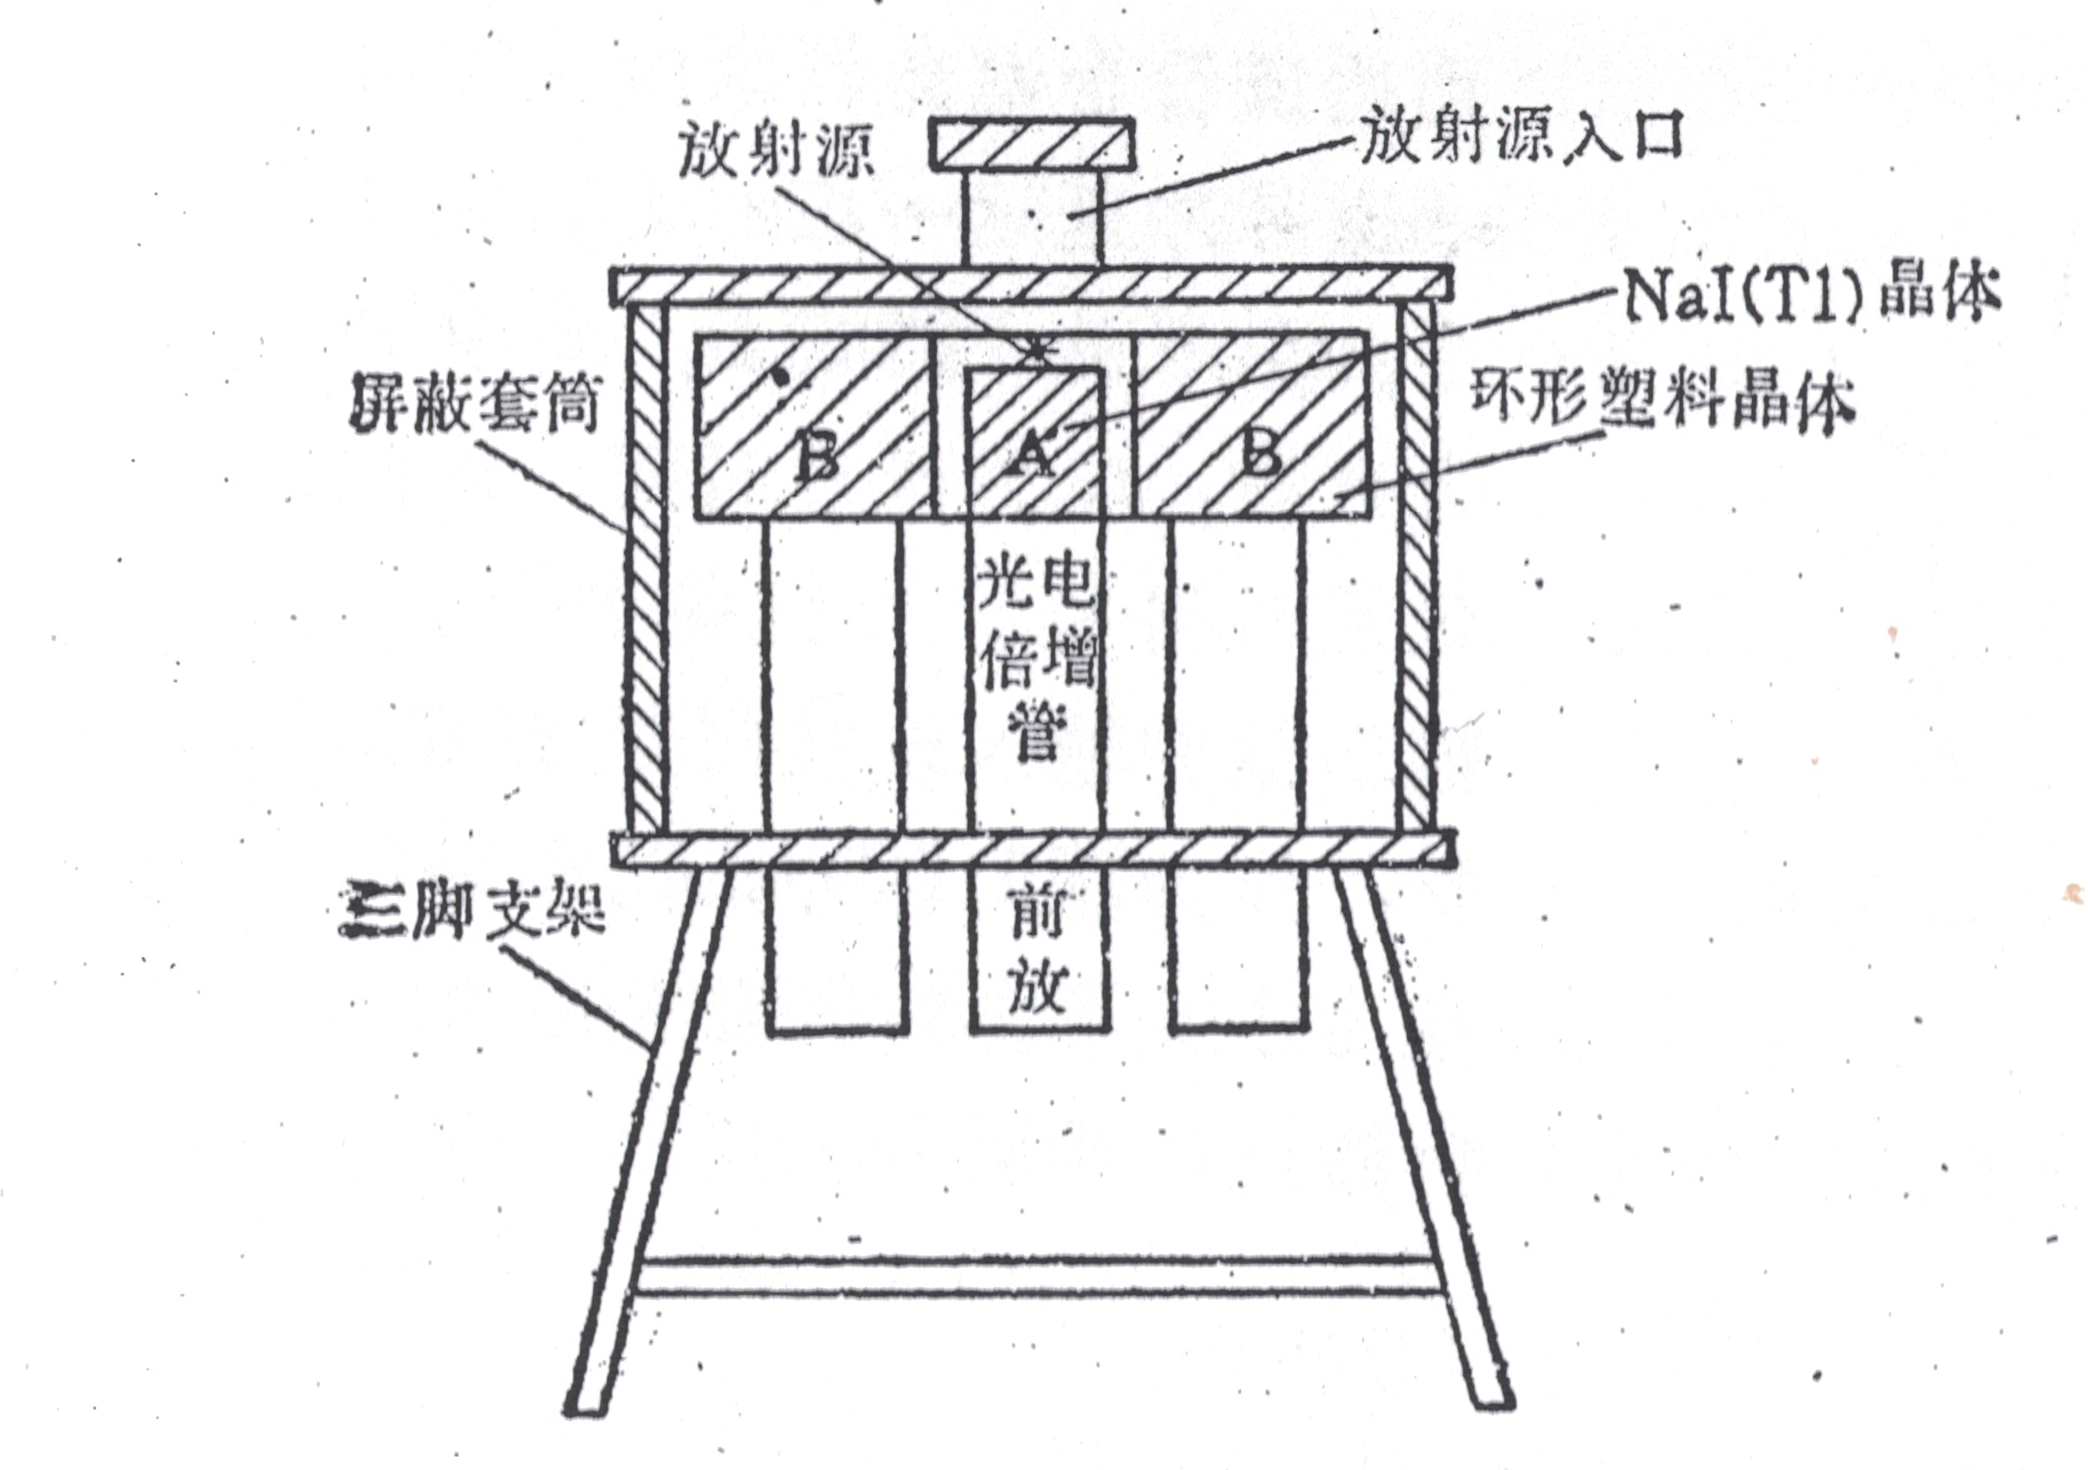
\includegraphics[width=0.45\textwidth]{yiqi.png}
\\
\xiaowu\song 图~1\begin{minipage}[t]{75mm} \quad 探测器结构示意图。\\[-1mm]\wuhao
\end{minipage}
\end{center}
\begin{center}
   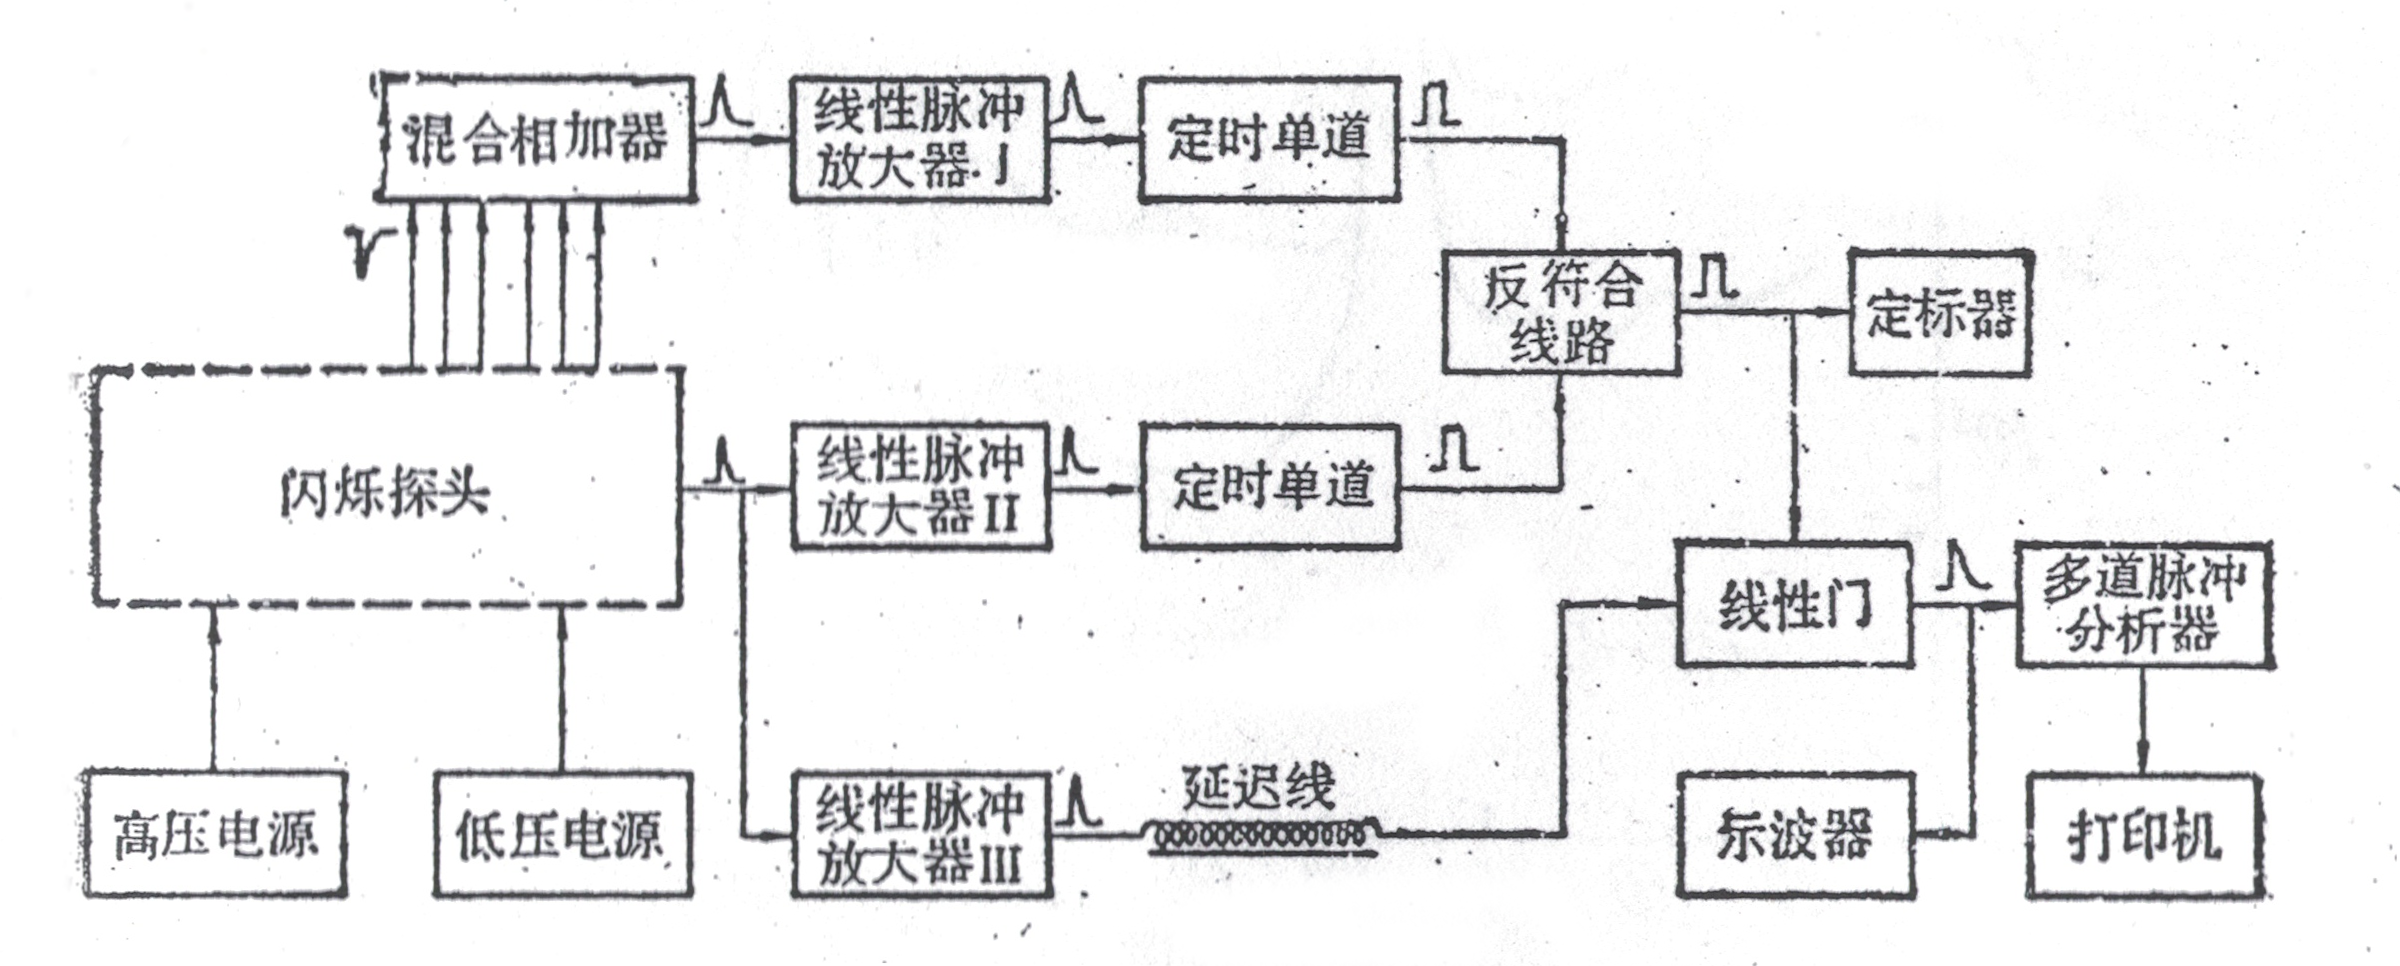
\includegraphics[width=0.45\textwidth]{jiexian.png}
\\
\xiaowu\song 图~2\begin{minipage}[t]{75mm} \quad 探测器电子学示意图。\\[-1mm]\wuhao
\end{minipage}
\end{center}

图1中,A是主探测器,探头由NaI(Ti)晶体,光电倍增管和前置放大器组成。B是反符合探测器,探头由一块环形塑料闪烁体包围NaI(Ti)晶体,五个光电倍增管和五个前置放大器组成。当$\gamma$射线进入晶体A时,康普顿散射后的光子被B记录,将A,B记录的脉冲分别输入线性脉冲放大器,然后将两路脉冲输入反符合电路的分析道和反符合道,则反符合电路输出的脉冲已排出了有时间关联的事件,即消除了主探测器A中发生的康普顿散射事件。

反符合屏蔽全吸收谱仪的实验装置如图2所示。

反符合方法可以用来排除同时事件,利用法符合方法可以将上述康普顿效应中反冲电子的事件和散射光子产生的事件从记录事件中除去,从而减少了反冲电子产生的脉冲数,从而达到降低康普顿电子的目的。

在测量的过程中,由于电子线路的延迟,同时事件不能同时到达发符合电路,只要把其中的快的一道延迟一段时间即可。实验中可通过测量N-td曲线,由此选定延迟时间。在此条件下将反符合输出脉冲输入到线性门电路的输入端,作为开门脉冲。门电路的另一输入端作为主探测器的待分析脉冲。
\section{实验内容和结果}
首先调节主放大器,调节其电压到681V, 峰值约为6.40V,此时的放大倍数约为4.12倍。

然后调节外围放大器的电压和放大倍数,使得他们的3s计数在大约1000到2000之间。

调节完成后测量$N_c-t_D$曲线,曲线如下图所示:

\begin{center}
   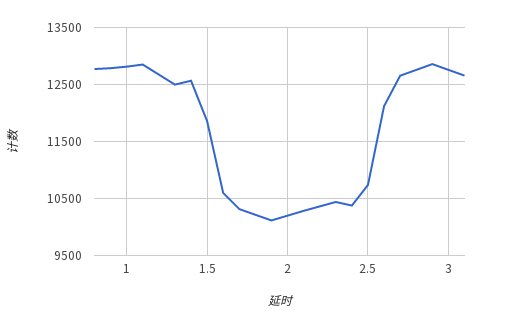
\includegraphics[width=0.45\textwidth]{1.png}
\\
\xiaowu\song 图~3\begin{minipage}[t]{75mm} \quad $N_c-t_D$曲线。测量时间为30s,延时单位为$\mu s$\\[-1mm]\wuhao
\end{minipage}
\end{center}

从曲线中可以明显的看出来发生反符合时候的低谷。下降沿和上升沿半高位置分别在1.52$\mu s$和2.55$\mu s$处。

随后需要调节进入反符合的两路的单道阈值,发现在取0.5V时候效果最好,此时最低计数约占最高计数的81.8\%.

然后是调节到达现行门的延时时间,调节标准为保持信号的主要特征,但是又不能有太长的后沿,从而减少死时间,提高计数。

然后就可以测量$^{137}$Cs的$\gamma$能谱了。用多道测量加入反符合和不含反符合的能谱,测量时间为40分钟,测量结果如下:

\begin{center}
   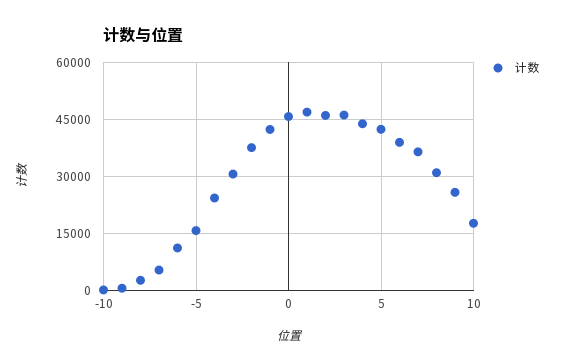
\includegraphics[width=0.45\textwidth]{2.png}
\\
\xiaowu\song 图~4\begin{minipage}[t]{75mm} $^{137}$Cs的$\gamma$能谱\quad \\[-1mm]\wuhao
\end{minipage}
\end{center}

随后就可以计算相关的参数。

首先是无反复和的能谱:

\begin{enumerate}
	\item 峰道址 548
	\item 峰计数 3822
	\item 峰半高宽 42.5
	\item 分辨率 7.8\%
	\item 康普顿坪面积 (358-388)28400
	\item 坪平均计数 946.7
	\item 谷面积 (449-479)9818
	\item 谷平均计数 327.3
	\item 峰康比 4.04
	\item 峰谷比 11.68
\end{enumerate}

然后是有反复和的能谱:

\begin{enumerate}
	\item 峰道址 545
	\item 峰计数 3836
	\item 峰半高宽 43.2
	\item 分辨率 7.9\%
	\item 康普顿坪面积 (358-388)23505
	\item 坪平均计数 783.5
	\item 谷面积 (449-479)7879
	\item 谷平均计数 262.6
	\item 峰康比 4.90
	\item 峰谷比 14.61
\end{enumerate}

可以明显的看出加入反符合后提高了峰康比和峰谷比。

\section{参考文献}

\noindent
[1] Peking Unviersity, Fudan University \ Nuclear Experment
\ Nuclear Publishing House, 1989 (in Chinese)

\noindent
 (北京大学,复旦大学.\ 原子核实验\ 原子能出版社,\ 1989)

\end{multicols}

\newpage

\clearpage
%\end{CJK*}
\end{document}

